\documentclass[aspectratio=169,12pt]{beamer}

% ---------------------------------------------------------------------------
% Beamer presentation: LLM-Based Session Recommendation
% Replace "Your Name" and the institute text before presenting.
% ---------------------------------------------------------------------------

\usetheme{Boadilla}
\usecolortheme{dove}
\usefonttheme{professionalfonts}
\setbeamertemplate{navigation symbols}{}

\usepackage[T1]{fontenc}
\usepackage[utf8]{inputenc}
\usepackage{amsmath,amssymb}
\usepackage{array,booktabs,tabularx,multirow}
\usepackage{graphicx}
\usepackage{hyperref}
\usepackage{listings}
\usepackage{ragged2e}
\usepackage{xcolor}
\usepackage{tikz}
\usetikzlibrary{arrows.meta,calc,fit,positioning,shapes.geometric}

% Palette
\definecolor{DeepBlue}{HTML}{143D59}
\definecolor{Teal}{HTML}{087E8B}
\definecolor{Orange}{HTML}{F28F3B}
\definecolor{SoftBlue}{HTML}{EAF2F8}
\definecolor{SoftTeal}{HTML}{E8F6F3}
\definecolor{SoftOrange}{HTML}{FFF3E8}
\definecolor{Ink}{HTML}{263238}
\definecolor{Muted}{HTML}{607D8B}
\definecolor{LightGray}{HTML}{D9E2E8}
\definecolor{CodeBackground}{HTML}{F5F7F9}

\setbeamercolor{structure}{fg=DeepBlue}
\setbeamercolor{normal text}{fg=Ink,bg=white}
\setbeamercolor{frametitle}{fg=DeepBlue,bg=SoftBlue}
\setbeamercolor{title}{fg=DeepBlue}
\setbeamercolor{subtitle}{fg=Muted}
\setbeamercolor{block title}{fg=white,bg=DeepBlue}
\setbeamercolor{block body}{fg=Ink,bg=SoftBlue}
\setbeamercolor{block title alerted}{fg=white,bg=Orange}
\setbeamercolor{block body alerted}{fg=Ink,bg=SoftOrange}
\setbeamercolor{block title example}{fg=white,bg=Teal}
\setbeamercolor{block body example}{fg=Ink,bg=SoftTeal}
\setbeamerfont{frametitle}{series=\bfseries,size=\Large}
\setbeamerfont{title}{series=\bfseries,size=\Huge}
\setbeamerfont{subtitle}{size=\large}

\setbeamertemplate{footline}{%
  \leavevmode%
  \hbox{%
    \begin{beamercolorbox}[wd=.82\paperwidth,ht=2.6ex,dp=1.1ex,leftskip=1em]{author in head/foot}%
      \usebeamerfont{author in head/foot}\insertshorttitle
    \end{beamercolorbox}%
    \begin{beamercolorbox}[wd=.18\paperwidth,ht=2.6ex,dp=1.1ex,center]{date in head/foot}%
      \usebeamerfont{date in head/foot}\insertframenumber/\inserttotalframenumber
    \end{beamercolorbox}}%
}

\newcommand{\source}[1]{\vspace{0.35em}\par{\tiny\color{Muted}\textit{#1}}}
\newcommand{\key}[1]{\textcolor{Teal}{\textbf{#1}}}
\newcommand{\warn}[1]{\textcolor{Orange}{\textbf{#1}}}
\newcommand{\code}[1]{\texttt{\footnotesize #1}}

\lstset{
  basicstyle=\ttfamily\scriptsize,
  columns=fullflexible,
  keepspaces=true,
  frame=single,
  rulecolor=\color{LightGray},
  backgroundcolor=\color{CodeBackground},
  breaklines=true,
  showstringspaces=false,
  keywordstyle=\color{DeepBlue},
  commentstyle=\color{Muted}
}

\title[Prompt \& Context Sensitivity]{Quantifying Prompt and Semantic Context Sensitivity\\in LLM-Based Session Recommendation}
\subtitle{Experimental pipeline, current implementation, and preliminary evidence}
\author{Your Name}
\institute{Department / College}
\date{\today}

\begin{document}

% ---------------------------------------------------------------------------
\begin{frame}[plain]
\centering
\vspace{0.6cm}
{\color{DeepBlue}\bfseries\LARGE
Quantifying Prompt and Semantic Context Sensitivity\par}
\vspace{0.25cm}
{\color{DeepBlue}\bfseries\LARGE
in LLM-Based Session Recommendation\par}
\vspace{0.45cm}
{\color{Muted}\large
Experimental pipeline, current implementation, and preliminary evidence\par}
\vfill
{\large Your Name\par}
\vspace{0.15cm}
{\normalsize Department / College\par}
{\normalsize \today\par}
\end{frame}

\section{Motivation and research question}

\begin{frame}{Presentation roadmap}
\begin{enumerate}
  \item Why prompt stability is a recommendation problem.
  \item How the dataset and evaluation unit are constructed.
  \item How the fixed LLM experiment is implemented.
  \item What the five-example pilot shows so far.
  \item What remains before a defensible research conclusion.
\end{enumerate}
\end{frame}

\begin{frame}{The problem: recommendation quality is not enough}
\begin{alertblock}{Central research problem}
An LLM-based recommender can change its ranking even when the user history,
candidate items, model, and decoding settings are unchanged.
\end{alertblock}

\vspace{0.4em}
\begin{itemize}
  \item A small wording change may move the correct item from the top five to
        much lower in the list.
  \item Additional context may help the model, or may distract it.
  \item A single accuracy score hides this instability.
\end{itemize}

\begin{block}{The question behind the project}
Does the recommender respond to the user's evidence, or does it respond too
strongly to how the evidence is described?
\end{block}
\end{frame}

\begin{frame}{Why this problem matters}
\begin{columns}[T]
\column{0.48\linewidth}
\begin{block}{For users and systems}
\begin{itemize}
  \item Inconsistent recommendations reduce trust.
  \item Prompt edits during deployment can silently change behavior.
  \item Invalid output can break an otherwise useful pipeline.
\end{itemize}
\end{block}

\column{0.48\linewidth}
\begin{block}{For research}
\begin{itemize}
  \item Results are difficult to reproduce if prompts are underspecified.
  \item Improvements may come from wording rather than model capability.
  \item Average HR/NDCG does not reveal ranking agreement.
\end{itemize}
\end{block}
\end{columns}

\vspace{0.5em}
\centering
\Large\textcolor{DeepBlue}{Reliability is a property to measure, not an assumption.}
\end{frame}

\begin{frame}{What is session-based recommendation?}
\begin{center}
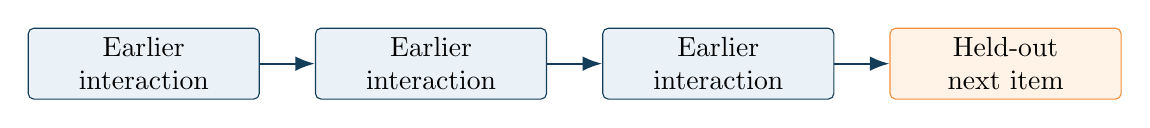
\begin{tikzpicture}[
  node distance=0.55cm and 0.7cm,
  box/.style={draw=DeepBlue, rounded corners=2pt, fill=SoftBlue,
              minimum height=0.9cm, text width=2.7cm, align=center},
  arrow/.style={-{Latex[length=2.5mm]}, thick, DeepBlue}
]
\node[box] (h1) {Earlier\\interaction};
\node[box, right=of h1] (h2) {Earlier\\interaction};
\node[box, right=of h2] (h3) {Earlier\\interaction};
\node[box, right=of h3, fill=SoftOrange, draw=Orange] (target) {Held-out\\next item};
\draw[arrow] (h1) -- (h2);
\draw[arrow] (h2) -- (h3);
\draw[arrow] (h3) -- (target);
\end{tikzpicture}
\end{center}

\vspace{0.5em}
\begin{itemize}
  \item The model receives a sequence of recent user--item interactions.
  \item It predicts which item is most likely to appear next.
  \item In this project, MovieLens ratings are converted into chronological
        session-like sequences.
\end{itemize}

\source{The project treats each eligible user's chronological rating history as a next-item session example.}
\end{frame}

\begin{frame}{Why LLM recommenders introduce extra uncertainty}
\begin{columns}[T]
\column{0.31\linewidth}
\begin{block}{Classical model}
\centering
Interactions\\
$\downarrow$\\
Learned representation\\
$\downarrow$\\
Ranking
\end{block}

\column{0.31\linewidth}
\begin{block}{LLM model}
\centering
Interactions\\
$+$\\
Prompt wording\\
$+$\\
Item context
\end{block}

\column{0.31\linewidth}
\begin{block}{New failure surface}
\centering
Different wording\\
$\Rightarrow$\\
Different reasoning\\
$\Rightarrow$\\
Different ranking
\end{block}
\end{columns}

\vspace{0.6em}
\begin{itemize}
  \item The LLM must understand both the recommendation task and the output
        protocol.
  \item The model can produce a valid but poor ranking, or an invalid response
        that cannot be evaluated.
\end{itemize}
\end{frame}

\begin{frame}{Research questions}
\begin{enumerate}
  \item \textbf{RQ1 -- Wording:} How much does the ranking change when the
        scoring instruction is rephrased?
  \item \textbf{RQ2 -- Semantic context:} How much does the ranking change when
        item information is presented differently?
  \item \textbf{RQ3 -- Reliability:} Do some conditions create more parsing or
        request failures?
  \item \textbf{RQ4 -- Reproducibility:} Are observed differences large enough
        to matter beyond random or sampling variation?
\end{enumerate}

\begin{exampleblock}{Current implementation status}
RQ1 is implemented through four wording variants. RQ2, full-scale evaluation,
ranking-stability statistics, and confidence intervals are the next stages.
\end{exampleblock}
\end{frame}

\section{Relationship to prior work}

\begin{frame}{The closest reference paper}
\begin{block}{Paper focus}
\emph{A Reproducibility Analysis of PO4ISR: Diagnosing and Mitigating Semantic
Drift in LLM-Based Session Recommendation}
\end{block}

\begin{columns}[T]
\column{0.48\linewidth}
\textbf{What the paper investigates}
\begin{itemize}
  \item Reproduction of PO4ISR.
  \item Cross-domain behavior on ML-1M, Games, and Bundle.
  \item Numerical ambiguity and parsing failures.
  \item Prompt overfitting across semantic domains.
\end{itemize}

\column{0.48\linewidth}
\textbf{What the paper proposes}
\begin{itemize}
  \item Deterministic index-based output.
  \item Reflexive cross-domain prompt fusion.
  \item Gemini 2.0 Flash as the reasoning engine.
  \item HR/NDCG benchmarking with 20-item pools.
\end{itemize}
\end{columns}

\source{Tiwari, Rekha, and Mundotiya, arXiv:2605.18780v1, 2026; provided PDF.}
\end{frame}

\begin{frame}{How this project relates to the paper}
\small
\begin{columns}[T]
\column{0.46\linewidth}
\begin{exampleblock}{Shared foundation}
\begin{itemize}
  \item LLM-based session recommendation.
  \item MovieLens-1M as a core dataset.
  \item Candidate pools of 20 items.
  \item Chronological next-item evaluation.
  \item HR and NDCG metrics.
  \item Reproducibility and prompt robustness.
\end{itemize}
\end{exampleblock}

\column{0.46\linewidth}
\begin{block}{Different contribution}
\begin{itemize}
  \item The paper proposes a robustness enhancement.
  \item This project measures sensitivity under controlled conditions.
  \item The same sessions and candidates are reused across prompt variants.
  \item Only one experimental factor is changed at a time.
  \item The local Qwen model and exact configuration are frozen.
\end{itemize}
\end{block}
\end{columns}

\vspace{0.5em}
\centering
\textcolor{DeepBlue}{This is a controlled extension, not a duplicate of PO4ISR++.}
\end{frame}

\begin{frame}{Similarity: the same reliability problem}
\begin{alertblock}{Common research motivation}
Both studies examine whether an LLM-based session recommender remains reliable
when the recommendation task is expressed through natural-language prompts.
\end{alertblock}

\begin{columns}[T]
\column{0.48\linewidth}
\begin{exampleblock}{Shared problem setting}
\begin{itemize}
  \item Predict the user's next item from a session history.
  \item Use semantic reasoning over item titles and metadata.
  \item Treat reproducibility as a research requirement.
  \item Investigate prompt-driven ranking changes.
\end{itemize}
\end{exampleblock}

\column{0.48\linewidth}
\begin{block}{Shared evaluation ideas}
\begin{itemize}
  \item MovieLens-1M is a common benchmark domain.
  \item Candidate sets contain 20 items.
  \item Evaluation is time-aware rather than purely random.
  \item HR/NDCG measure next-item ranking quality.
  \item Invalid or unparseable outputs are reliability evidence.
\end{itemize}
\end{block}
\end{columns}

\source{Comparison based on Tiwari, Rekha, and Mundotiya, arXiv:2605.18780v1, 2026; provided paper.}
\end{frame}

\begin{frame}{Similarity and difference in methodology}
\scriptsize
\begin{tabularx}{\linewidth}{@{}p{0.20\linewidth}p{0.36\linewidth}X@{}}
\toprule
\textbf{Aspect} & \textbf{Reference paper} & \textbf{This project}\\
\midrule
Research goal & Reproduce PO4ISR and improve robustness against semantic drift. & Measure the isolated effect of prompt wording and semantic context.\\[0.35em]
Datasets & ML-1M, Games, and Bundle. & MovieLens-1M as the controlled starting domain.\\[0.35em]
LLM & Gemini 2.0 Flash. & Locally hosted Qwen2.5-3B-Instruct through Ollama.\\[0.35em]
Candidate/evaluation & 20-item pools with HR and NDCG benchmarking. & 20-item fixed pools with HR@1/5/10 and NDCG@5/10.\\[0.35em]
Output protocol & Index-based candidate positions to reduce numerical ambiguity. & JSON score list, followed by deterministic ranking and strict validation.\\[0.35em]
Prompt strategy & Reflexive cross-domain prompt fusion. & Four wording variants, followed by planned context variants.\\
\bottomrule
\end{tabularx}

\vspace{0.45em}
\begin{block}{Key interpretation}
The shared components make the studies comparable; the controlled differences
define the specific contribution of this project.
\end{block}

\source{Reference-paper details: Tiwari et al., arXiv:2605.18780v1, 2026, pp. 1--8. Project details: current experiment contract and implementation.}
\end{frame}

\begin{frame}{How this project extends the reference paper}
\begin{columns}[T]
\column{0.47\linewidth}
\begin{block}{What the paper establishes}
\begin{itemize}
  \item Prompt-based session recommendation has reproducibility risks.
  \item Long or semantically complex contexts can cause drift.
  \item Numerical item names can produce output and parsing failures.
  \item Deterministic indexing and cross-domain fusion can improve robustness.
\end{itemize}
\end{block}

\column{0.47\linewidth}
\begin{exampleblock}{What this project adds}
\begin{itemize}
  \item A one-factor-at-a-time sensitivity protocol.
  \item The same sessions and candidates reused across conditions.
  \item Frozen model, decoding, output schema, parser, and evaluator.
  \item Direct measurement of target-rank movement and ranking stability.
\end{itemize}
\end{exampleblock}
\end{columns}

\vspace{0.55em}
\begin{alertblock}{Positioning in one sentence}
The paper focuses on diagnosing and mitigating semantic drift; this project
quantifies how much a fixed recommender changes when its wording or context is
perturbed.
\end{alertblock}

\source{Reference-paper claims: Tiwari et al., arXiv:2605.18780v1, 2026. The extension describes this project's planned full analysis.}
\end{frame}

\begin{frame}{The research gap addressed by this project}
\begin{tabularx}{\linewidth}{@{}p{0.30\linewidth}X@{}}
\toprule
\textbf{Existing emphasis} & \textbf{Gap for this study}\\
\midrule
Improve one prompt or fuse prompts &
Quantify the effect of wording itself.\\[0.4em]
Compare domains &
Separate semantic context from other changes.\\[0.4em]
Report average recommendation accuracy &
Report ranking changes and stability.\\[0.4em]
Use a successful output only &
Retain and count parsing failures.\\
\bottomrule
\end{tabularx}

\vspace{0.7em}
\begin{alertblock}{Planned contribution}
An auditable protocol for measuring prompt and semantic-context sensitivity
while the recommendation problem remains fixed.
\end{alertblock}
\end{frame}

\section{Experimental design}

\begin{frame}{Complete project pipeline}
\centering
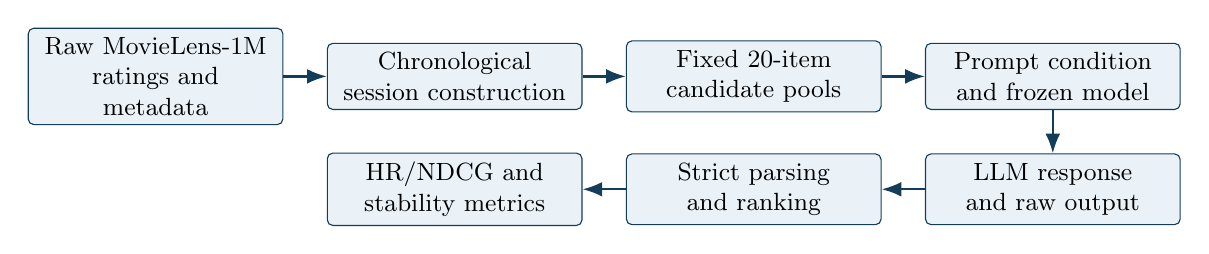
\begin{tikzpicture}[
  node distance=0.55cm,
  every node/.style={font=\small},
  stage/.style={draw=DeepBlue, rounded corners=2pt, fill=SoftBlue,
               minimum height=0.8cm, text width=3.0cm, align=center},
  arrow/.style={-{Latex[length=2.5mm]}, thick, DeepBlue}
]
\node[stage] (raw) {Raw MovieLens-1M\\ratings and metadata};
\node[stage, right=of raw] (data) {Chronological\\session construction};
\node[stage, right=of data] (pool) {Fixed 20-item\\candidate pools};
\node[stage, right=of pool] (prompt) {Prompt condition\\and frozen model};
\node[stage, below=of prompt] (llm) {LLM response\\and raw output};
\node[stage, left=of llm] (parse) {Strict parsing\\and ranking};
\node[stage, left=of parse] (metric) {HR/NDCG and\\stability metrics};
\draw[arrow] (raw) -- (data);
\draw[arrow] (data) -- (pool);
\draw[arrow] (pool) -- (prompt);
\draw[arrow] (prompt) -- (llm);
\draw[arrow] (llm) -- (parse);
\draw[arrow] (parse) -- (metric);
\end{tikzpicture}

\vspace{0.5em}
\begin{block}{Experimental principle}
The input session and candidate set stay fixed; the tested prompt factor changes.
\end{block}
\end{frame}

\begin{frame}{Dataset: MovieLens-1M}
\begin{table}
\centering
\small
\begin{tabular}{lr}
\toprule
\textbf{Prepared quantity} & \textbf{Current value}\\
\midrule
Ratings & 1,000,209\\
Users & 6,040\\
Distinct rated items & 3,706\\
Movie metadata rows & 3,883\\
Session examples & 6,040\\
Training ratings after target removal & 994,169\\
Candidate pools & 6,040\\
Candidates per pool & 20\\
\bottomrule
\end{tabular}
\end{table}

\begin{itemize}
  \item Movie titles and genres supply the item context.
  \item One final interaction is held out for each eligible user.
  \item The 5-example runs are engineering pilots; 6,040 examples are the
        planned full evaluation.
\end{itemize}
\end{frame}

\begin{frame}[fragile]{Chronological session construction}
\begin{block}{Definition}
For each user, sort interactions by timestamp and use the final interaction as
the held-out next-item target.
\end{block}

\begin{lstlisting}[language=Python]
for user_id, user_rows in ratings.groupby("user_id"):
    ordered = sort(user_rows, by=["timestamp", "item_id"])
    prefix = ordered.iloc[:-1]       # model input
    target = ordered.iloc[-1]        # hidden evaluation label
\end{lstlisting}

\begin{itemize}
  \item A deterministic item-ID tie-breaker handles equal timestamps.
  \item Users with fewer than the minimum history length are excluded.
  \item The target is never placed in the session prefix.
\end{itemize}
\end{frame}

\begin{frame}{One leave-one-out example}
\begin{center}
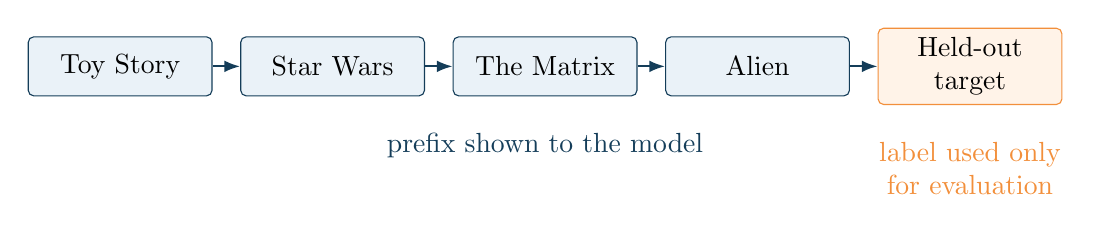
\begin{tikzpicture}[
  node distance=0.35cm,
  item/.style={draw=DeepBlue, fill=SoftBlue, rounded corners=2pt,
               minimum height=0.75cm, text width=2.1cm, align=center},
  target/.style={draw=Orange, fill=SoftOrange, rounded corners=2pt,
               minimum height=0.75cm, text width=2.1cm, align=center},
  arrow/.style={-{Latex[length=2mm]}, thick, DeepBlue}
]
\node[item] (a) {Toy Story};
\node[item, right=of a] (b) {Star Wars};
\node[item, right=of b] (c) {The Matrix};
\node[item, right=of c] (d) {Alien};
\node[target, right=of d] (e) {Held-out\\target};
\draw[arrow] (a) -- (b);
\draw[arrow] (b) -- (c);
\draw[arrow] (c) -- (d);
\draw[arrow] (d) -- (e);
\node[below=0.35cm of c, text width=5cm, align=center, text=DeepBlue]
  {prefix shown to the model};
\node[below=0.35cm of e, text width=2.6cm, align=center, text=Orange]
  {label used only for evaluation};
\end{tikzpicture}
\end{center}

\vspace{0.4em}
\begin{block}{Why this is important}
The model is evaluated on a realistic temporal task: predicting a future
interaction from past interactions, rather than memorizing a randomly selected
target.
\end{block}
\end{frame}

\begin{frame}{Candidate-pool construction}
\begin{columns}[T]
\column{0.52\linewidth}
\begin{block}{For every session}
\begin{enumerate}
  \item Start with the held-out target.
  \item Select 19 negative items using training-only popularity.
  \item Exclude items already in the prefix.
  \item Insert the target at a controlled position.
\end{enumerate}
\end{block}

\column{0.42\linewidth}
\begin{exampleblock}{Candidate list}
\centering
\code{[target, negative, negative, \ldots]}\\[0.5em]
\code{20 unique item IDs}\\[0.5em]
\code{target position: 0--19}
\end{exampleblock}
\end{columns}

\vspace{0.5em}
\begin{itemize}
  \item Candidate order is recorded and reused for every prompt condition.
  \item Target positions are balanced across positions 0 through 19.
\end{itemize}
\end{frame}

\begin{frame}{Leakage and validity controls}
\begin{tabularx}{\linewidth}{@{}p{0.30\linewidth}X@{}}
\toprule
\textbf{Control} & \textbf{Purpose}\\
\midrule
Chronological split &
Do not use future interactions as history.\\
Target excluded from prefix &
The model cannot see the answer in the session.\\
Training-only popularity &
The target does not influence negative sampling.\\
Fixed candidate order &
Position effects are controlled and reproducible.\\
Strict output validation &
Malformed responses are counted, not silently repaired.\\
\bottomrule
\end{tabularx}

\vspace{0.6em}
\centering
\Large\textcolor{DeepBlue}{Every trial must be auditable from input to metric.}
\end{frame}

\begin{frame}{Frozen LLM configuration}
\begin{table}
\centering
\small
\begin{tabular}{ll}
\toprule
\textbf{Setting} & \textbf{Frozen value}\\
\midrule
Provider & Ollama, OpenAI-compatible local endpoint\\
Model tag & \code{qwen2.5:3b-instruct}\\
Model ID & \code{357c53fb659c} (observed in the project contract)\\
Ollama version & \code{0.32.15} in the experiment contract\\
Temperature & 0\\
Top-p & 1\\
Maximum output tokens & 256\\
Output mode & JSON object with a \code{scores} list\\
Request timeout & 600 seconds\\
\bottomrule
\end{tabular}
\end{table}

\source{Before the full run, verify the model ID and Ollama version in the actual runtime and update the experiment contract if necessary.}
\end{frame}

\begin{frame}[fragile]{The prompt contract}
\begin{columns}[T]
\column{0.48\linewidth}
\textbf{Inputs held constant}
\begin{itemize}
  \item Session prefix and order.
  \item Candidate IDs, titles, and order.
  \item System/user message structure.
  \item Output schema and parser.
\end{itemize}

\column{0.48\linewidth}
\textbf{Output requirement}
\begin{lstlisting}
{
  "scores": [s_1, s_2, ..., s_20]
}
\end{lstlisting}
\begin{itemize}
  \item One finite score per candidate position.
  \item Every score must be in the range 0--100.
\end{itemize}
\end{columns}

\begin{block}{Design choice}
The LLM scores candidate positions; the program—not the LLM—creates the final
rank using a deterministic rule.
\end{block}
\end{frame}

\begin{frame}{Wording sensitivity conditions}
\begin{table}
\centering
\scriptsize
\begin{tabularx}{\linewidth}{@{}p{0.28\linewidth}X@{}}
\toprule
\textbf{Variant ID} & \textbf{Changed scoring instruction}\\
\midrule
\code{baseline\_scores\_v1} &
Neutral next-interaction relevance scoring.\\
\code{wording\_direct\_v1} &
Directly estimate which candidate the user will interact with next.\\
\code{wording\_preference\_v1} &
Match each candidate to the user's inferred preferences.\\
\code{wording\_detailed\_v1} &
Compare the complete history with each candidate carefully.\\
\bottomrule
\end{tabularx}
\end{table}

\vspace{0.5em}
\begin{alertblock}{Controlled comparison}
Only the three-line scoring instruction changes. Session, candidates, model,
decoding, format, parser, and evaluation code remain fixed.
\end{alertblock}
\end{frame}

\begin{frame}{Semantic-context sensitivity: the next factor}
\begin{table}
\centering
\small
\begin{tabular}{lll}
\toprule
\textbf{Condition} & \textbf{Information shown} & \textbf{Status}\\
\midrule
\code{context\_title\_v1} & Movie title only & Planned\\
\code{context\_genre\_v1} & Title plus MovieLens genres & Planned\\
\code{context\_rich\_v1} & Title, genre, and permitted metadata & Planned\\
\bottomrule
\end{tabular}
\end{table}

\begin{itemize}
  \item The same session and candidate pool must be reused across conditions.
  \item The target must not receive privileged information unavailable to other
        candidates.
  \item Add one context factor at a time so its effect is interpretable.
\end{itemize}

\begin{exampleblock}{Interpretation}
Wording changes the instruction. Semantic context changes the information
available to the model.
\end{exampleblock}
\end{frame}

\begin{frame}{One trial: from data to ranking}
\begin{enumerate}
  \item Load one chronological session example.
  \item Load its fixed 20-item candidate pool.
  \item Render the selected prompt variant.
  \item Send the request to the frozen local model.
  \item Save the raw response.
  \item Validate and parse the score list.
  \item Sort scores into a ranking using candidate position as a tie-breaker.
  \item Record the target rank and failure state.
\end{enumerate}

\vspace{0.5em}
\centering
\textcolor{DeepBlue}{One session + one condition + one response = one trial record}
\end{frame}

\begin{frame}{Parsing: converting LLM text into a ranking}
\begin{center}
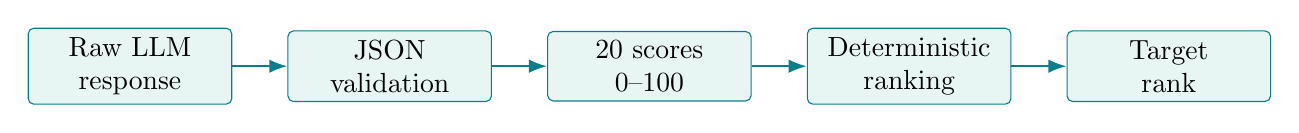
\begin{tikzpicture}[
  node distance=0.6cm and 0.7cm,
  stage/.style={draw=Teal, rounded corners=2pt, fill=SoftTeal,
                minimum height=0.75cm, text width=2.35cm, align=center},
  arrow/.style={-{Latex[length=2.3mm]}, thick, Teal}
]
\node[stage] (raw) {Raw LLM\\response};
\node[stage, right=of raw] (json) {JSON\\validation};
\node[stage, right=of json] (score) {20 scores\\0--100};
\node[stage, right=of score] (rank) {Deterministic\\ranking};
\node[stage, right=of rank] (target) {Target\\rank};
\draw[arrow] (raw) -- (json);
\draw[arrow] (json) -- (score);
\draw[arrow] (score) -- (rank);
\draw[arrow] (rank) -- (target);
\end{tikzpicture}
\end{center}

\begin{itemize}
  \item Scores are sorted in descending order.
  \item Ties are resolved by earlier candidate position.
  \item The target rank is used to compute HR and NDCG.
\end{itemize}
\end{frame}

\begin{frame}{What is a parsing failure?}
\begin{columns}[T]
\column{0.48\linewidth}
\begin{exampleblock}{Valid response}
\code{\{"scores": [85, 42, 91, \ldots]\}}\\[0.4em]
Exactly 20 finite numeric values in the range 0--100.
\end{exampleblock}

\column{0.48\linewidth}
\begin{alertblock}{Invalid response examples}
\begin{itemize}
  \item Extra explanation outside the JSON.
  \item Wrong key: \code{score} instead of \code{scores}.
  \item Fewer or more than 20 values.
  \item Text values, missing values, or scores outside 0--100.
\end{itemize}
\end{alertblock}
\end{columns}

\vspace{0.5em}
\begin{block}{Important distinction}
A parsing failure means the output cannot be evaluated. A valid but low-ranked
target is a recommendation failure, not a parsing failure.
\end{block}
\end{frame}

\begin{frame}[fragile]{The trial record preserves evidence}
\begin{lstlisting}
{
  "trial_id": "user-1::wording_direct_v1",
  "prompt_variant_id": "wording_direct_v1",
  "prefix_item_ids": [...],
  "candidate_item_ids": [...],
  "target_item_id": 48,
  "target_position_in_candidates": 0,
  "prompt": {...},
  "client_config": {...},
  "raw_response": "...",
  "ranked_item_ids": [...],
  "parse_success": true,
  "target_rank": 3
}
\end{lstlisting}

\begin{itemize}
  \item Raw and parsed information are both retained.
  \item A failed trial remains visible with an error reason.
\end{itemize}
\end{frame}

\section{Evaluation and implementation}

\begin{frame}{Metric 1: Hit Ratio}
\begin{block}{Definition}
\[
\mathrm{HR@k} =
\frac{1}{N}\sum_{i=1}^{N}
\mathbf{1}\bigl[\mathrm{rank}_i(\mathrm{target}) \leq k\bigr]
\]
\end{block}

\begin{itemize}
  \item HR@1 asks: was the target the first recommendation?
  \item HR@5 asks: did the target appear in the top five?
  \item HR@10 asks: did the target appear in the top ten?
\end{itemize}

\begin{exampleblock}{Interpretation}
If HR@5 is 0.40, the target appeared in the top five for 40\% of valid trials.
\end{exampleblock}
\end{frame}

\begin{frame}{Metric 2: NDCG and planned stability metrics}
\begin{block}{NDCG for one held-out target}
\[
\mathrm{NDCG@k} =
\begin{cases}
\dfrac{1}{\log_2(1+\mathrm{rank})}, & \mathrm{rank}\leq k\\[0.6em]
0, & \mathrm{rank}>k
\end{cases}
\]
\end{block}

\begin{itemize}
  \item NDCG rewards a target more strongly when it is near rank 1.
  \item The current evaluator calculates NDCG@5 and NDCG@10.
  \item Planned stability measures include Kendall's $\tau$, top-$k$ Jaccard
        overlap, and target-rank change between variants.
\end{itemize}
\end{frame}

\begin{frame}[fragile]{Implementation map: which file does what?}
\begin{lstlisting}
EXPERIMENT_SPEC.md
  experiment question and frozen settings

scripts/prepare_movielens.py
  download, preprocess, and write JSONL data

src/llm_session_reco/movielens.py
  load ratings, sessions, targets, and candidate pools

scripts/run_baseline.py
  orchestrate trials and save raw/parsed outputs

src/llm_session_reco/prompts.py
  render baseline and wording variants
src/llm_session_reco/llm_client.py
  call Ollama through the local API
src/llm_session_reco/parser.py
  validate scores and create rankings

scripts/evaluate_baseline.py
  calculate HR/NDCG
scripts/compare_variants.py
  compare prompt-condition metric files
\end{lstlisting}
\end{frame}

\begin{frame}[fragile]{Execution order from start to finish}
\begin{lstlisting}[language=bash]
# 1. Activate the project environment
cd C:\Users\user\Desktop\projectt
.\.venv\Scripts\Activate.ps1

# 2. Prepare MovieLens data
python scripts\prepare_movielens.py

# 3. Start Ollama separately, then run a small pilot
python scripts\run_baseline.py --provider chat-completions \
  --model qwen2.5:3b-instruct \
  --base-url http://localhost:11434/v1 \
  --temperature 0 --top-p 1 --max-tokens 256 --limit 5

# 4. Evaluate the trial JSONL
python scripts/evaluate_baseline.py --input <trials.jsonl> \
  --output <metrics.json>

# 5. Compare all prompt variants
python scripts/compare_variants.py
\end{lstlisting}
\end{frame}

\begin{frame}{Pilot protocol completed so far}
\begin{table}
\centering
\small
\begin{tabular}{ll}
\toprule
\textbf{Pilot property} & \textbf{Value}\\
\midrule
Dataset & MovieLens-1M\\
Examples per condition & 5\\
Candidate pool & 20 items\\
Model & Qwen2.5 3B Instruct\\
Temperature / top-p & 0 / 1\\
Output format & Strict JSON scores\\
Wording conditions & 4\\
Valid trials per condition & 5/5\\
Parsing/request failures & 0/0 in the recorded pilot outputs\\
\bottomrule
\end{tabular}
\end{table}

\begin{alertblock}{Status}
This validates the engineering pipeline. It is not yet a final estimate of
MovieLens performance.
\end{alertblock}
\end{frame}

\begin{frame}{Pilot results: wording conditions}
\begin{table}
\centering
\scriptsize
\begin{tabular}{lrrrrr}
\toprule
\textbf{Variant} & \textbf{HR@1} & \textbf{HR@5} & \textbf{HR@10}
& \textbf{NDCG@5} & \textbf{NDCG@10}\\
\midrule
\code{baseline\_scores\_v1} & 0.20 & 0.20 & 0.40 & 0.200 & 0.263\\
\code{wording\_direct\_v1} & 0.40 & 0.40 & 0.60 & 0.400 & 0.460\\
\code{wording\_preference\_v1} & 0.00 & 0.40 & 0.40 & 0.212 & 0.212\\
\code{wording\_detailed\_v1} & 0.00 & 0.00 & 0.40 & 0.000 & 0.142\\
\bottomrule
\end{tabular}
\end{table}

\source{Source: current project pilot metric files; 5 valid trials per wording condition. Values are preliminary.}
\end{frame}

\begin{frame}{What the pilot suggests}
\begin{columns}[T]
\column{0.48\linewidth}
\begin{exampleblock}{Evidence of sensitivity}
\begin{itemize}
  \item HR@1 ranges from 0.00 to 0.40 across equivalent wording conditions.
  \item HR@5 ranges from 0.00 to 0.40.
  \item The direct wording condition is strongest in this tiny pilot.
\end{itemize}
\end{exampleblock}

\column{0.48\linewidth}
\begin{alertblock}{What it does not prove}
\begin{itemize}
  \item It does not establish a general winner.
  \item Five examples are too few for statistical conclusions.
  \item Semantic-context effects have not yet been measured.
\end{itemize}
\end{alertblock}
\end{columns}

\vspace{0.6em}
\centering
\textcolor{DeepBlue}{The pilot justifies the full controlled experiment.}
\end{frame}

\begin{frame}{What is completed}
\begin{tabularx}{\linewidth}{@{}p{0.62\linewidth}p{0.25\linewidth}@{}}
\toprule
\textbf{Deliverable} & \textbf{Status}\\
\midrule
Python environment and package structure & Complete\\
MovieLens-1M download and loader & Complete\\
Chronological leave-one-out examples & Complete\\
Training-only popularity candidate pools & Complete\\
Fixed 20-item candidate lists & Complete\\
Ollama-compatible LLM client & Complete\\
Strict score parser and failure recording & Complete\\
HR/NDCG evaluator & Complete\\
Four wording variants & Complete\\
Five-example pilot runs and comparison & Complete\\
\bottomrule
\end{tabularx}
\end{frame}

\begin{frame}{What remains before the final conclusion}
\begin{enumerate}
  \item Run all 6,040 examples for every wording condition.
  \item Implement and run semantic-context conditions.
  \item Add ranking-stability metrics.
  \item Use paired bootstrap confidence intervals or paired tests.
  \item Report valid, parsing-failure, and request-failure rates separately.
  \item Freeze and record the final model/runtime version and dataset hashes.
  \item Write the results, limitations, and reproducibility appendix.
\end{enumerate}

\begin{block}{Decision rule}
Do not select a prompt only because it wins a five-example pilot. Select it
only after full-scale accuracy and stability analysis.
\end{block}
\end{frame}

\begin{frame}{Threats to validity and how to control them}
\begin{tabularx}{\linewidth}{@{}p{0.36\linewidth}X@{}}
\toprule
\textbf{Threat} & \textbf{Control}\\
\midrule
Small pilot size &
Use all 6,040 examples and report uncertainty.\\
Model-specific conclusions &
Clearly scope the claim to Qwen2.5 3B, or add another model later.\\
Temperature zero may not guarantee exact identity &
Record model ID, runtime version, raw outputs, and repeat trials where feasible.\\
Prompt and context may change together &
Use one-factor-at-a-time variants.\\
Accuracy may hide ranking instability &
Add rank correlation, top-$k$ overlap, and target-rank movement.\\
Outdated configuration notes &
Use one experiment contract and verify it before the full run.\\
\bottomrule
\end{tabularx}
\end{frame}

\section{Interpretation and contribution}

\begin{frame}{Possible outcomes and their meaning}
\begin{table}
\centering
\small
\begin{tabularx}{\linewidth}{@{}p{0.30\linewidth}X@{}}
\toprule
\textbf{Observed result} & \textbf{Interpretation}\\
\midrule
High accuracy, high agreement &
The prompt condition is both effective and stable.\\
High accuracy, low agreement &
The prompt may work, but the recommender is fragile.\\
Low accuracy, high agreement &
The model is consistently making a poor prediction.\\
High parsing-failure rate &
The output interface or prompt is not operationally reliable.\\
Context improves accuracy and agreement &
The added information is useful and robust.\\
Context improves accuracy but reduces agreement &
The information helps some sessions but creates sensitivity.\\
\bottomrule
\end{tabularx}
\end{table}
\end{frame}

\begin{frame}{Expected scientific contribution}
\begin{columns}[T]
\column{0.31\linewidth}
\begin{block}{Measurement}
Turn vague prompt sensitivity into measurable changes in target rank, HR,
NDCG, and ranking agreement.
\end{block}

\column{0.31\linewidth}
\begin{block}{Method}
Provide a repeatable one-factor-at-a-time protocol with fixed sessions,
candidates, model, decoding, and parser.
\end{block}

\column{0.31\linewidth}
\begin{block}{Practice}
Show when an LLM recommender can be trusted, and when prompt changes require
re-evaluation.
\end{block}
\end{columns}

\vspace{0.7em}
\centering
\textcolor{DeepBlue}{The contribution is an evidence-based reliability analysis,
not merely another prompt.}
\end{frame}

\begin{frame}{How to position the work in a paper}
\begin{block}{Suggested positioning}
The reference paper demonstrates that LLM-based session recommenders can suffer
from parsing errors, prompt overfitting, and semantic-domain drift. This study
extends that direction through a controlled sensitivity analysis: it holds the
session, candidate pool, model, decoding configuration, and parser fixed, then
measures the isolated effects of prompt wording and semantic context on
recommendation quality and ranking stability.
\end{block}

\vspace{0.6em}
\begin{itemize}
  \item Cite the PO4ISR reproducibility paper as the closest prior work.
  \item Do not claim that the current five-example pilot is final evidence.
  \item Make the full 6,040-example experiment and statistical analysis the
        basis of the paper's main claims.
\end{itemize}
\end{frame}

\begin{frame}{Conclusion}
\begin{enumerate}
  \item LLM session recommendation may be sensitive to prompt wording and
        semantic context.
  \item This project measures that sensitivity under controlled conditions.
  \item The data pipeline prevents temporal leakage and fixes candidate pools.
  \item The model, decoding settings, output schema, and parser are frozen.
  \item The pilot already shows meaningful wording differences, but it is only
        an engineering validation.
  \item The final research result requires the full dataset, context variants,
        stability metrics, and statistical uncertainty.
\end{enumerate}

\vspace{0.7em}
\centering
\Large\textcolor{DeepBlue}{Same recommendation problem. Different prompt.
How much does the answer move?}
\end{frame}

\begin{frame}{References and project artifacts}
\footnotesize
\begin{thebibliography}{9}
\bibitem{tiwari2026}
A. Tiwari, K. N. L. Rekha, and R. K. Mundotiya.
\newblock \emph{A Reproducibility Analysis of PO4ISR: Diagnosing and Mitigating
Semantic Drift in LLM-Based Session Recommendation}.
\newblock arXiv preprint arXiv:2605.18780v1, 2026.

\bibitem{movielens}
F. M. Harper and J. A. Konstan.
\newblock The MovieLens datasets: History and context.
\newblock \emph{ACM Transactions on Interactive Intelligent Systems}, 5(4), 2015.

\bibitem{project}
Current project artifacts:
\code{EXPERIMENT\_SPEC.md}, \code{src/llm\_session\_reco/},
\code{scripts/}, and \code{tests/}.
\end{thebibliography}

\vspace{0.4em}
\centering
\textcolor{Muted}{The pilot values shown in this deck are from the project's
recorded five-example metric outputs.}
\end{frame}

\end{document}
